\documentclass{article}

\usepackage[english]{babel}

% Set page size and margins
% Replace `letterpaper' with `a4paper' for UK/EU standard size
\usepackage[letterpaper,top=2cm,bottom=2cm,left=3cm,right=3cm,marginparwidth=1.75cm]{geometry}

% Useful packages
\usepackage{amsmath}
\usepackage{graphicx}
\usepackage{xcolor}
\usepackage{minted}
\usepackage{graphicx}
\usepackage{hyperref}
\usepackage{listings}
\definecolor{LightGray}{gray}{0.9}
\usepackage[colorlinks=true, allcolors=blue]{hyperref}

\lstset{frame=tb,
  language=Java,
  aboveskip=3mm,
  belowskip=3mm,
  showstringspaces=false,
  columns=flexible,
  basicstyle={\small\ttfamily},
  numbers=none,
  numberstyle=\tiny\color{gray},
  keywordstyle=\color{blue},
  commentstyle=\color{dkgreen},
  stringstyle=\color{mauve},
  breaklines=true,
  breakatwhitespace=true,
  tabsize=3
}
\title{COP290 Lab-3}
\author{Fouriers}
\date{}
\begin{document}
\maketitle


\section{Overview}
\textbf{queriKorner} is a question-and-answer website that allows users to ask and answer questions.
Users can search relevant questions and can filter all questions by tags.
Questions and answers can be sorted based on votes and time.
Users can also upvote and downvote questions and answers.
Users can see their profiles and can edit their details.
Users can also see top users and top questions.
Each user has a reputation score calculated based on the votes on their questions and answers.
\section{Baadal VM link}

We have hosted our website on Baadal VM. The link to our website is
\href{http://10.17.9.97:8061/}{http://10.17.9.97:8061/}

\section{Site Map}

\begin{figure}[h]
    \centering
    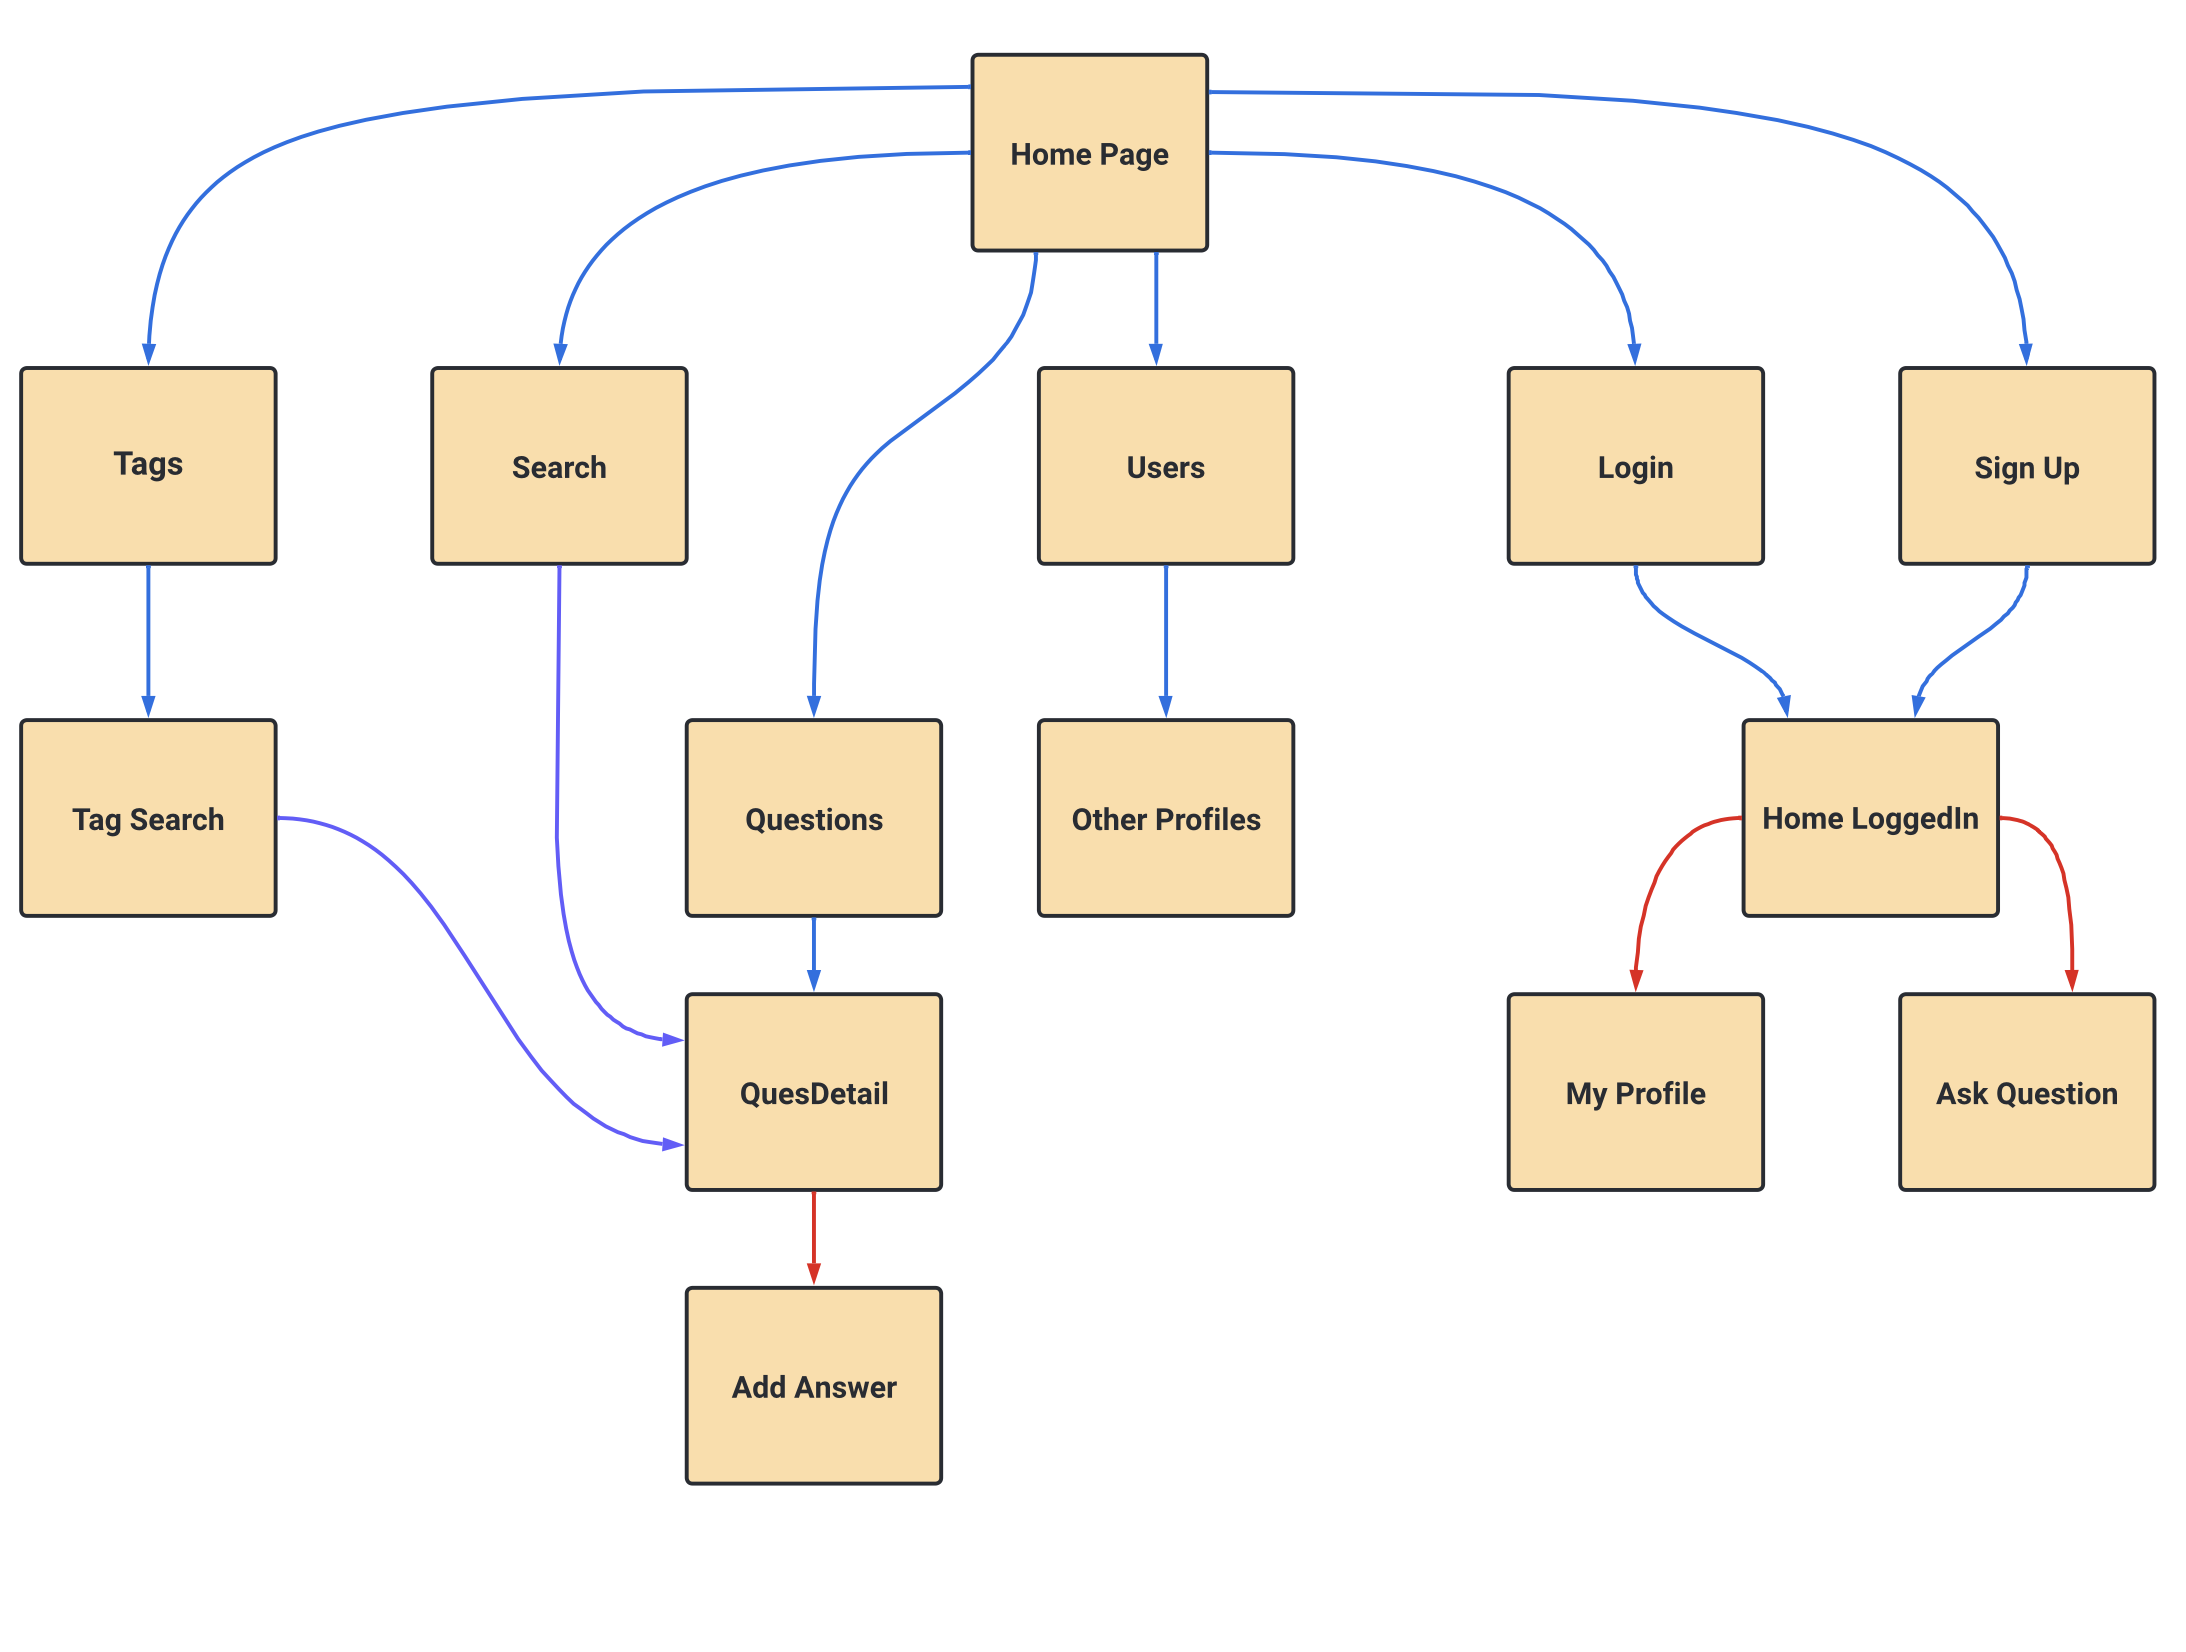
\includegraphics[width=13cm]{sitemap.png}
    \caption[short]{Site Map}
    \end{figure}

\newpage


\begin{itemize}
    \item Here the red arrows represent the flow of the website for a logged in user and the blue arrows represent the flow of the website for any user.
    \item Additionally user can logout from any page if logged in to go back to home page.
\end{itemize}
\section{ER Diagram}



\begin{figure}[h]
    \centering
    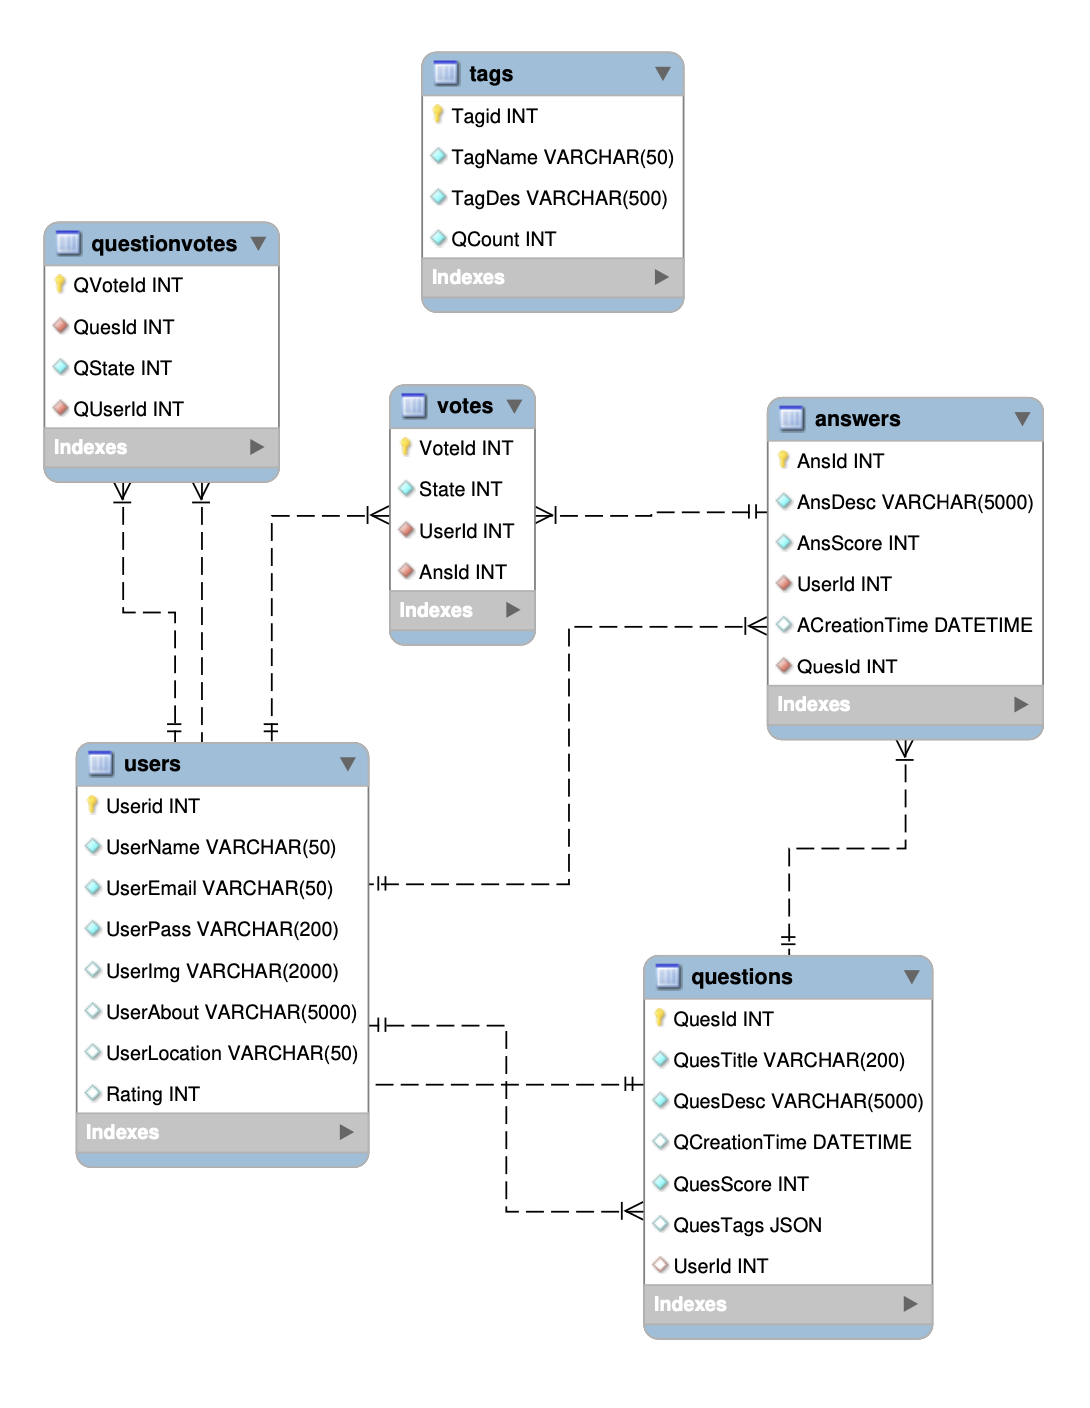
\includegraphics[width=11cm]{ERD.png}
    \caption[short]{ER Diagram}
    \end{figure}




\section{Github Link}



\section{API descriptions}


The following are the APIs that we have implemented in our project:

\begin{itemize}
    \item \textcolor{red}{\textbf{\textfractionsolidus}} \\ This renders the home page of the website.
    It contains the list of recently asked questions which is fetched from question database. It also contains a truncated list of top users and top questions which is fetched from users and questions database.
    \item Authentication APIs
    \begin{itemize}
        \item \textcolor{red}{\textbf{ \textfractionsolidus login}}  \\ This is the login API. It takes values of \textcolor{blue}{( Username , Password )} from the user and checks if the username and password are valid or not. If the username and password are valid, then the user is logged in and redirected to the home page. If the username and password are invalid, then the user is redirected to the login page again.
        \item \textcolor{red}{\textbf{ \textfractionsolidus signup}} \\ This is the signup API. It takes values of \textcolor{blue}{( Username , email , password )} from the user and creates a new user in the database. It also checks if the username is unique or not and if the email is valid or not.
        \item \textcolor{red}{\textbf{ \textfractionsolidus logout}} \\ This is the logout API. It logs out the user and redirects to the login page.
    \end{itemize}
    
    \item Tag related APIs:
    \begin{itemize}
        \item \textcolor{red}{\textbf{\textfractionsolidus tags\textfractionsolidus \textless string:sort\textgreater }} \\ This API fetches all the tags from the database and displays them in the form of cards and applying Pagination. The tags can be sorted based on the number of questions  \textcolor{blue}{( QCount )}  and lexicographically \textcolor{blue}{( TagName )}.
    \end{itemize}
    \item User details related APIs:
    \begin{itemize}
        \item \textcolor{red}{\textbf{\textfractionsolidus users\textfractionsolidus \textless string:sort\textgreater }} \\ This API fetches all the users from the database and displays them in the form of cards and applying Pagination. The users can be sorted based on the reputation score \textcolor{blue}{( RepScore )} and lexicographically \textcolor{blue}{( UserName )}.
        \item \textcolor{red}{\textbf{\textfractionsolidus myprofile}} \\ This API fetches the details of the logged in user from the database and displays them in the html page.
        \item \textcolor{red}{\textbf{\textfractionsolidus editprofie}} \\ This API fetches the details \textcolor{blue}{( UserImage , UserLocation , UserEmail )} of the logged in user from the form submitted by the user and the values are updated in the database. 
        \item \textcolor{red}{\textbf{\textfractionsolidus changepasswd}} \\ This API fetches the details \textcolor{blue}{( OldPassword , NewPassword , ConfirmPassword )} of the logged in user from the form submitted by the user and the values are updated in the database if the OldPassword matches with the password in the database and the NewPassword and ConfirmPassword match.
        \item \textcolor{red}{\textbf{\textfractionsolidus otherprofile\textfractionsolidus \textless int:id\textgreater}} \\ This API fetches the details of the user with the given id from the database and displays them in a html page which shows limited information.
    \end{itemize}
    \item Question related APIs
    \begin{itemize}
        \item \textcolor{red}{\textbf{\textfractionsolidus questions\textfractionsolidus \textless string:sort\textgreater }} \\ This API fetches all the questions from the database and displays them in the form of cards with Pagination. The questions can be sorted based on the number of votes \textcolor{blue}{( QuesVotes )} and lexicographically \textcolor{blue}{( QuesTitle )}.
        \item \textcolor{red}{\textbf{\textfractionsolidus question\textfractionsolidus \textless int:id\textgreater }} \\ This API fetches the details of the question with the given id from the database and displays them in a html page.
        \item \textcolor{red}{\textbf{\textfractionsolidus ask}} \\ This API fetches the details \textcolor{blue}{( QuesTitle , QuesBody , QuesTags )} of the question from the form submitted by the user and the values are inserted in the database.
        \item \textcolor{red}{\textbf{\textfractionsolidus answer\textfractionsolidus \textless int:id\textgreater }} \\ This API fetches the values of the answer from the form submitted by the user and the values are inserted in the database. The id refers to Question Id to which the answer is being posted.
        \item \textcolor{red}{\textbf{\textfractionsolidus search}} \\ This API fetches the search query from the form submitted by the user and relevant values are searched in the database and displayed in the html page.
    \end{itemize}
    \item Voting APIs
    \begin{itemize}
        \item \textcolor{red}{\textbf{\textfractionsolidus upvoteAns\textfractionsolidus \textless int:id\textgreater }} \\ This API fetches the id of the answer from the url and increments the value of AnsVotes in the database of answers , answervotes and user reputation .
        \item \textcolor{red}{\textbf{\textfractionsolidus downvoteAns\textfractionsolidus \textless int:id\textgreater }} \\ This API fetches the id of the answer from the url and decrements the value of AnsVotes in the database of answers , answervotes and user reputation .
        \item \textcolor{red}{\textbf{\textfractionsolidus QuesUpvote\textfractionsolidus \textless int:id\textgreater }} \\ This API fetches the id of the question from the url and increments the value of QuesVotes in the database of questions , questionvotes and user reputation.
        \item \textcolor{red}{\textbf{\textfractionsolidus QuesDownvote\textfractionsolidus \textless int:id\textgreater }} \\ This API fetches the id of the question from the url and decrements the value of QuesVotes in the database of questions , questionvotes and user reputation.
    \end{itemize}
    
    
\end{itemize}
\section{CI/CD Test Coverage}
\begin{lstlisting}
(env) Dhruvs-MacBook-Air:test dhruvgupta$ make coverage
python3 test.py
Test 1 completed
Test 2 completed
Test 3 completed
Test 4 completed
Test 5 completed
Test 6 completed
Test 8 completed
python -m coverage run -m unittest
Test 8 completed
.Test 1 completed
.Test 6 completed
.Test 3 completed
.Test 7 completed
.Test 4 completed
.Test 2 completed
.Test 5 completed
.
----------------------------------------------------------------------
Ran 8 tests in 0.058s

OK
python -m coverage report -m
Name      Stmts   Miss  Cover   Missing
---------------------------------------
test.py      53      8    85%   69-76
---------------------------------------
TOTAL        53      8    85%
\end{lstlisting}

\section{Design decisions}

\begin{itemize}
    \item We decided to use \textcolor{red}{Bootstrap 5} instead of other tools such as ReactJS to make front end of the website because importing and using ReactJS would have made the website heavy and slow and importing Bootstrap 5 with CDN is much easier and faster.
    \item We used  \textcolor{red}{\mintinline{python}|spacy|}  for natural language processing API for search api instead of other APIs such as NLTK because we found spacy easier to use.
    \item We decided to use \textcolor{red}{datetime module of python} to print time in format such as "2 minutes ago"  instead of directly using string . We also used \textcolor{red}{python re module} to check if the string is a valid email or not instead of relying on html for it.
    \item We used module \textcolor{red}{ \mintinline{python}|flask_paginate|} to use pagination in all users and all question pages   \textcolor{red}{\mintinline{python}|flask_bcrypt|} to hash passwords and \textcolor{red}{\mintinline{python}|flask_login|} to manage user sessions.
    \item We assigned a \textcolor{red}{limited number of characters} in the title and body of the question and answer to prevent the user from entering a very long string which would have made the website look bad. This made some data from kaggle dataset unusable.
    \item Instead of storing whole images in database we stored a \textcolor{red}{image link} in database .
    \item We decided to use \textcolor{red}{seperate tables for \textcolor{blue}{( questionUpvotes )} and \textcolor{blue}{( answerUpvotes )}} instead of storing them in the same table because it was convinient
\end{itemize}

\section{ML API}
We have used Spacy which is an advanced natural language processing library to sort results on the basis of relevancy.
The method takes user's query as an input and tokenize it.
Similarity Score of query is calculated with all the questions in the database which is a value between 0 and 1.
The score is calculated using the cosine similarity metric, which is a measure of the similarity between two non-zero vectors in a high-dimensional space.
The API then sorts the relevant questions in descending order of similarity score.
\subsection{Cosine Similarity}
Cosine similarity is a measure of similarity between two non-zero vectors of an inner product space that measures the cosine of the angle between them.
The cosine of 0° is 1, and it is less than 1 for any other angle.
It is thus a judgment of orientation and not magnitude: two vectors with the same orientation have a cosine similarity of 1, two vectors at 90° have a similarity of 0, and two vectors diametrically opposed have a similarity of -1, independent of their magnitude.
Cosine similarity is particularly used in positive space, where the outcome is neatly bounded in [0,1].
\subsection{Using SpaCy for natural language processing}
Spacy is an open-source software library for advanced natural language processing, written in the programming languages Python and Cython. We used \mintinline{python3}|nlp = spacy.load("en_core_web_md")| to load a medium english core. And using data from \textcolor{blue}{( QuesTitle )} in questions database we trained it to give similarity score with user's query.
\section{Unique Features}
\subsection{MathJax \& Quill Text Editor}
We have used MathJax to render mathematical equations in the questions and answers. We have also used Quill text editor to make the text editor more user friendly.

\begin{figure}[h]
    \centering
    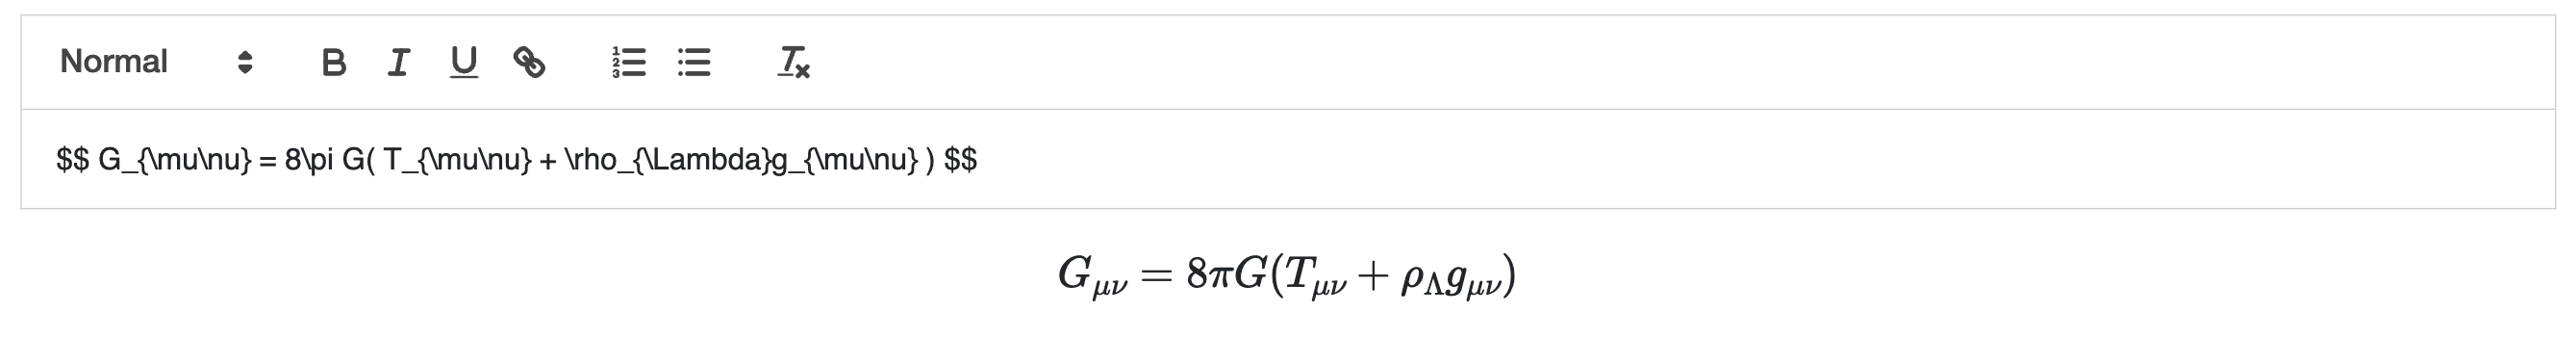
\includegraphics[width=13cm]{MathJax1.png}
    \end{figure}


\subsection{Password Encryption}
We have used \textcolor{red}{\mintinline{python}|flask_bcrypt|} to hash passwords and \textcolor{red}{\mintinline{python}|flask_login|} to manage user sessions.


We have used Bcrypt as a password hashing function.
At the time of signup , Bcrypt generates a random salt and concatenate it with the password entered by the user. The salt is then stored alongside the hashed password in the database.
At the time of login , Bcrypt takes two arguments password entered by the user and hashed password retrieved from the database. The salt stored in the hashed password is used to hash the entered password and resulting hash is compared to stored hash.
\section{Challenges}
\begin{itemize}
    \item \textbf{Lack of Experience :} None of our team members were familiar with web development and we had to learn everything from scratch. We had to learn HTML, CSS, Javascript, Bootstrap, Flask, MySQL, Figma etc. in a short period of time.
    \item \textbf{Figma :} We were not able to use figma to make the frontend of the website using figma plugins like locofy and anima . So we started making the frontend design from scratch manually using HTML and CSS and also made use of some components from  bootstrap 5 to make the frontend of the website.
    \item \textbf{Database :} We were not able to add datetime in mysql database. Then we changed the date time format in csv file and imported it in mysql database. There were some non ascii characters in csv files which were not getting imported in mysql database. We figured out a way to remove those characters from csv files and then imported it in mysql database.
    \item \textbf{Baadal VM :} We were getting difficulties in downloading various modules and libraries to run our website. We found other alternatives to download those modules and libraries and then we were able to run our website on baadal vm.
    \item \textbf{bootstrap :} We were not able to place different placeholders and cards of bootstrap properly. We tried different ways to place them properly and finally we were able to place them properly.
\end{itemize}

\section{Limitations / FutureWork}
\begin{itemize}
    \item \textbf{2 Factor Authentication :} 2 factor authentication can be implemented in our website. A verification code can be sent to the user's email id and the user can enter that code to verify his/her account. This will make the website more secure. Forgot Password functionality can also be provided using the above feature.
    \item \textbf{Offensive Text recognition :} ML API can be used to recognize offensive text and the user can be warned about the same. The user can be banned from the website if he/she continues to post offensive text.
    \item \textbf{Moderator Access :} A moderator can be given access to delete users and questions. This will help in maintaining the quality of the website.
    \item \textbf{Comments :} Comments can be added to the answers and questions. This will help in making the website more interactive.
    \item \textbf{Edit/Delete Questions/Answers :} The user can be given the option to edit/delete his/her questions and answers. This will help in making the website more user friendly.
\end{itemize}
\section{Video Link}
Here is a link to the video: \url{https://drive.google.com/file/d/1R9tvtAgXhbHHi50Yh8Vy-l3f6PY_ttxj/view?usp=sharing}
\section{Token Distribution}

\begin{table}[h]
    \centering
    \begin{tabular}{|c|c|c|c|}
    \hline
    \textbf{S.No.} & \textbf{Team member} & \textbf{Entry No.} & \textbf{Token} \\ \hline
    1              & Hemang Sidana        & 2021CS10078        & 10             \\ \hline
    2              & Dhruv Gupta          & 2021CS50125        & 10             \\ \hline
    3              & Rounik Roushan       & 2021CS10243        & 10             \\ \hline
    4              & Priyanshu Ranjan     & 2021CS10575        & 10             \\ \hline
    \end{tabular}
    \caption{Token Distribution}
    \label{tab:token-split}
    \end{table}


\end{document}